\documentclass{beamer}

\usepackage{beamerthemesplit}

\usetheme{Boadilla} 

\usepackage[utf8]{inputenc}
\usepackage[T1]{fontenc}
\usepackage[utf8]{vietnam}
\usepackage[english]{babel}
\usepackage{calc}
\usepackage{ifthen}
\usepackage{tikz}
\usepackage{eurosym}

\usepackage{alltt}

\usepackage{verbatim}

\usepackage{mdframed}

\usepackage[algoruled,vlined,noend]{algorithm2e}
%\SetKwIF{Si}{SinonSi}{Sinon}{si}{}{sinon si}{sinon}{}
%\SetKwFor{Pour}{pour}{}{}
%\SetKwFor{RepeterNFois}{répéter}{fois}{}
%\SetKwFor{TantQue}{tant que}{}{}%
%\SetKwFor{PourChaque}{pour chaque}{}{}%

\usepackage{CJKutf8}

\usepackage[overlap, CJK]{ruby}
\usepackage{CJKulem}

\renewcommand{\rubysep}{-0.2ex}

\newenvironment{SChinese}{%
  \CJKfamily{gbsn}%
  \CJKtilde
  \CJKnospace}{}
\newenvironment{TChinese}{%
  \CJKfamily{bsmi}%
  \CJKtilde
  \CJKnospace}{}
\newenvironment{Japanese}{%
  \CJKfamily{min}%
  \CJKtilde
  \CJKnospace}{}
\newenvironment{Korean}{%
  \CJKfamily{mj}}{}
  
  
\DeclareMathOperator*{\argmax}{arg\!\max}
  
\newcommand{\cntext}[1]{\begin{CJK}{UTF8}{}\begin{Japanese}#1\end{Japanese}\end{CJK}}

\pgfdeclareimage[height=0.8cm]{logo}{img/getalp}
\pgfdeclareimage[height=1.5cm]{logobig}{img/getalp} 

\logo{\pgfuseimage{logo}}

\title[Disambiguating Translations in DBnary]{Attaching Translations to Proper Lexical Senses in DBnary}
%\subtitle{Wiktionnaire, RDF, Linked Data: une colonne vertébrale pour le lexique ?}
\author[Tchechmedjiev et al. \hspace{-2mm}]{Andon Tchechmedjiev, Gilles Sérasset, Jérôme Goulian, Didier Schwab}
\institute[\fontsize{1.8mm}{1mm}\selectfont GETALP-LIG, Grenoble]{GETALP-LIG, Univ Grenoble Alpes, France}
\titlegraphic{\pgfuseimage{logobig}}
\date{May 27, 2014}

% Delete this, if you do not want the table of contents to pop up at
% the beginning of each subsection:
\AtBeginSection[]
{
  \begin{frame}<beamer>
    \frametitle{}
    \tableofcontents[currentsection]
  \end{frame}
}

\begin{document}

\frame{\titlepage}


\section{Context: DBnary dataset}

\frame{\frametitle{What is Dbnary?}

\begin{center}
	     \includegraphics<1->[width=.8\linewidth]{img/logos/logos.pdf}
\end{center}


\only<1>{Lexical data extracted from 12 different Wiktionary language editions\\
$\rightarrow$ 2 more in alpha version.}

\only<2>{Extracted data is available as Linked Data\\
$\rightarrow$ structure using LEMON, LEXINFO and few BDnary extensions.}

	
}

\frame{
	\frametitle{LEMON and Dbnary}

     \includegraphics<1>[width=0.95\linewidth]{img/lemon-core.png}
     \includegraphics<2>[width=0.95\linewidth]{img/dbnary-lemon-xtension.pdf}

}

\frame{  
\frametitle{Dbnary: an example}

     \includegraphics<1>[width=\linewidth]{img/cat_struct}
     \includegraphics<2>[width=\linewidth]{img/cat_syn}
     \includegraphics<3>[width=\linewidth]{img/cat_translations}

}

\frame{  
\frametitle{Dataset Size (as of today)}

\begin{table}[htb]
\begin{tabular}{lrrrr}
 & \textbf{Vocables} & \textbf{Entries} & \textbf{Senses} & \textbf{Translations}\\
 \hline
\textbf{English}	&	523,300	&	562,538	&	454,285	&	1,366,385	\\
\textbf{French}	&	285,497	&	299,444	&	388,642	&	514,525	\\
\textbf{Greek}	&	242,470	&	248,107	&	140,190	&	58,952	\\
\textbf{German}	&	212,226	&	215,808	&	104,556	&	396,376	\\
\textbf{Russian}	&	149,534	&	152,488	&	152,394	&	381,641	\\
\textbf{Turkish}	&	66,830	&	67,820	&	99,148	&	68,416	\\
\textbf{Spanish}	&	57,385	&	60,438	&	88,022	&	116,912	\\
\textbf{Finnish}	&	54,376	&	55,783	&	64,931	&	125,615	\\
\textbf{Portuguese}	&	42,503	&	46,553	&	82,900	&	269,516	\\
\textbf{Italian}	&	32,735	&	35,313	&	46,367	&	63,711	\\
\textbf{Japanese}	&	21,547	&	26,267	&	30,720	&	93,161	\\
\textbf{Bulgarian}	&	18,792	&	18,823	&	18,299	&	13,925	\\
\hline
\textbf{Total}	&	1,707,195	&	1,789,382	&	1,670,454	&	3,469,135

\end{tabular}
\caption{Number of resources by type and language, sorted by number of lexical entries.}\label{globalsize}
\end{table}
}

\frame{  
\frametitle{Dataset Size (as of today)}
\begin{table}[htb]
\begin{tabular}{lrrrrrr}
	&	\textbf{syn}	&	\textbf{ant}	&	\textbf{hyper}	&	\textbf{hypo}	&	\textbf{holo}	&	\textbf{mero}\\
\textbf{German}	&	123,550	&	55,158	&	95,962	&	81,467	&	0	&	0	\\
\textbf{English}	&	32,147	&	7,056	&	1,210	&	1,234	&	0	&	114	\\
\textbf{French}	&	32,089	&	6,929	&	9,673	&	3,776	&	1,914	&	978	\\
\textbf{Russian}	&	25,844	&	10,134	&	42,955	&	5,250	&	0	&	0	\\
\textbf{Bulgarian}	&	17,623	&	34	&	0	&	0	&	0	&	0	\\
\textbf{Spanish}	&	15,562	&	1,602	&	784	&	565	&	0	&	0	\\
\textbf{Italian}	&	10,148	&	3,718	&	0	&	0	&	0	&	0	\\
\textbf{Greek}	&	5,439	&	1,553	&	0	&	0	&	0	&	0	\\
\textbf{Japanese}	&	4,002	&	1,631	&	10	&	18	&	0	&	0	\\
\textbf{Portuguese}	&	3,395	&	621	&	6	&	4	&	0	&	0	\\
\textbf{Turkish}	&	3,219	&	242	&	484	&	166	&	0	&	0	\\
\textbf{Finnish}	&	2,654	&	0	&	0	&	0	&	0	&	0	\\
\hline
\textbf{Total}	&	275,672	&	88,678	&	151,084	&	92,480	&	1,914	&	1,092	
\end{tabular}
\caption{Number of lexicon-semantic relations. Languages are sorted according to the number of synonym.}\label{nymsize}
\end{table}
}

% \frame{  
% \frametitle{Dataset Size (as of today)}
% \begin{table}[htb]
% \begin{tabular}{lrrrrrrrrrrrrr}\tiny
% \textbf{Source/Target}  & \textbf{deu} & \textbf{ell} & \textbf{eng} & \textbf{fin} & \textbf{fra} & \textbf{ita} & \textbf{por} & \textbf{rus}& \textbf{others} & \textbf{Total} & \textbf{\# of target languages}\\
% \textbf{eng} & 62501 & 23794 & 1 & 74938 & 57959 & 37467 & 30256 & 74837 & 764710 & 1126463 & 1143\\
% \textbf{fra} & 34608 & 7063 & 74687 & 7589 & 12 & 18806 & 17784 & 7783 & 296624 & 464956 & 952\\
% \textbf{deu} & 0 & 2675 & 81015 & 4947 & 67143 & 41485 & 8872 & 17354 & 248401 & 471892 & 355\\
% \textbf{rus} & 23056 & 3295 & 48559 & 3966 & 14776 & 12643 & 5567 & 0 & 206709 & 318571 & 490\\
% \textbf{ell} & 2242 & 2 & 10090 & 1056 & 8436 & 1470 & 1149 & 1315 & 29892 & 55652 & 246\\
% \textbf{fin} & 8046 & 918 & 30103 & 0 & 6700 & 3856 & 2196 & 7997 & 58912 & 118728 & 329\\
% \textbf{por} & 7000 & 2816 & 11284 & 4607 & 8720 & 7096 & 4 & 4396 & 179142 & 225065 & 695\\
% \textbf{ita} & 4619 & 506 & 17539 & 925 & 4461 & 75 & 1219 & 938 & 27514 & 57796 & 315\\
% \end{tabular}
% \caption{Number of translations from/to the 8 currently extracted languages. Source languages are sorted according to their number of lexical entries. Target languages are sorted by their ISO 639-3 language code. The number of different target languages is also given.}\label{tradsize1}
% \end{table}
% }

% \frame{  
% \frametitle{Dataset Size (as of today)}
% \begin{table}[htb]
% \begin{tabular}{lrrrrrr}
% \textbf{Source/Target}  & \textbf{por} & \textbf{rus}& \textbf{others} & \textbf{Total} & \textbf{\# of lang}\\
% \textbf{eng} & 30256 & 74837 & 764710 & 1126463 & 1143\\
% \textbf{fra} & 17784 & 7783 & 296624 & 464956 & 952\\
% \textbf{deu} & 8872 & 17354 & 248401 & 471892 & 355\\
% \textbf{rus} &  5567 & 0 & 206709 & 318571 & 490\\
% \textbf{ell} &  1149 & 1315 & 29892 & 55652 & 246\\
% \textbf{fin} &  2196 & 7997 & 58912 & 118728 & 329\\
% \textbf{por} &  4 & 4396 & 179142 & 225065 & 695\\
% \textbf{ita} &  1219 & 938 & 27514 & 57796 & 315\\
% \end{tabular}
% \caption{Number of translations from/to the 8 currently extracted languages. Source languages are sorted according to their number of lexical entries. Target languages are sorted by their ISO 639-3 language code. The number of different target languages is also given.}\label{tradsize2}
% \end{table}
% }

\section{Attaching Translation to their Proper Lexical Sense}

\subsection{Problem}

\frame{  
\frametitle{The problem}

\only<1>{\vfill\begin{mdframed}\includegraphics[width=\linewidth]{img/dbnarystrc1}\end{mdframed}}
\only<2>{\vfill\begin{mdframed}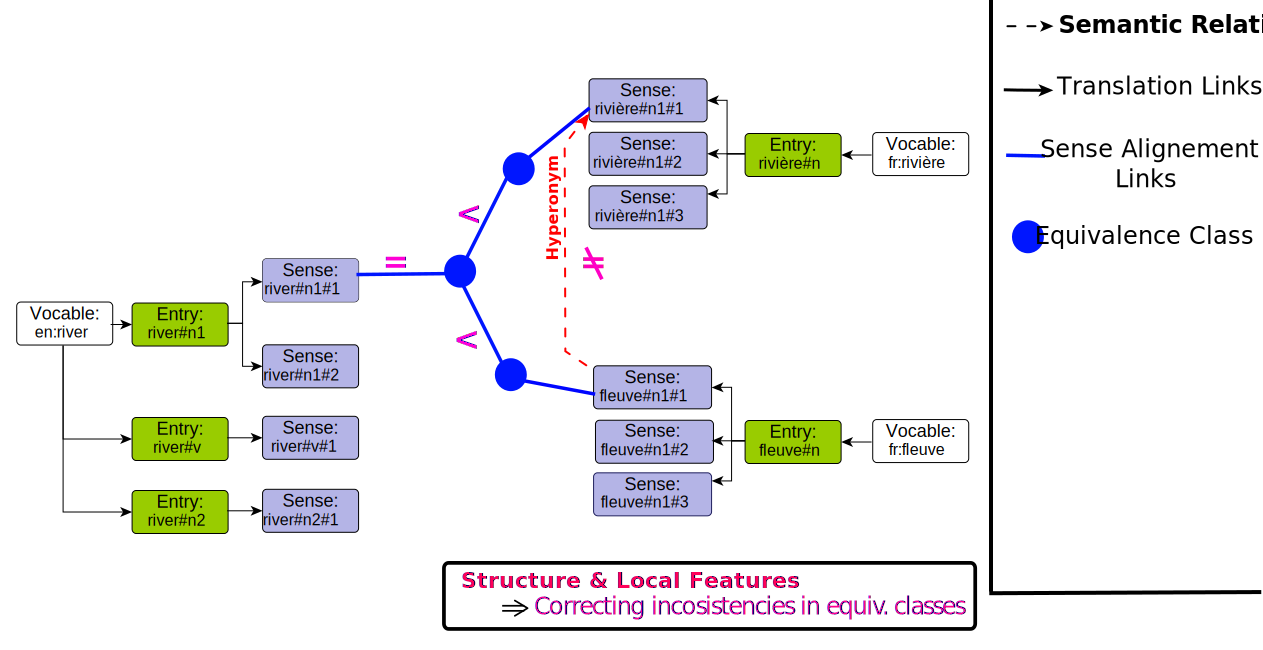
\includegraphics[width=\linewidth]{img/dbnarystrc2}\end{mdframed}}
% \begin{overprint}
% \onslide<3>
% \begin{center}
% \[T, \mbox{ the set of translation relations}\]
% \[
% \forall T_i \in T, S=Senses(Source(T_i)): 
% \]
% \[
%   M_S = \max_{S_k\in S}(Score((Gloss(T_i),Def(S^k))),
% \]
% \vfill
% \[
% \argmax_{S_i\in S}^\delta \{Score(Gloss(T_i),Def(S^k))\}=
% \]
% \[
% \{S^k\in S|  M_S > Score((Gloss(T_i),Def(S^k)) > M_S-\delta \}
% \]
% \vfill
% \end{center}
% \end{overprint}	
}

\frame{  
\frametitle{Some Cues}

As an example, the English \texttt{LexicalEntry} \emph{frog} contains 8 word senses, defined as follows:

\begin{tiny}\begin{enumerate}
\item A small tailless amphibian of the order Anura that typically hops
\item The part of a violin bow (or that of other similar string instruments such as the viola, cello and contrabass) located at the end held by the player, to which the horsehair is attached
\item (Cockney rhyming slang) Road. Shorter, more common form of frog and toad
\item The depression in the upper face of a pressed or handmade clay brick
\item An organ on the bottom of a horse’s hoof that assists in the circulation of blood
\item The part of a railway switch or turnout where the running-rails cross (from the resemblance to the frog in a horse’s hoof)
\item An oblong cloak button, covered with netted thread, and fastening into a loop instead of a button hole.
\item The loop of the scabbard of a bayonet or sword. 
\end{enumerate}\end{tiny}

Translations of this entry are divided in 4 groups corresponding to: ``\emph{amphibian}'', ``\emph{end of a string instrument’s bow}'', ``\emph{organ in a horse’s foot}'' and ``\emph{part of a railway}''. This is what we call the \textbf{glosses}.

}

\frame{  
\frametitle{Different languages, different cues}

\begin{itemize}
	\item English language edition uses glosses to annotate translations.
	\item German language edition uses the sense number to annotate translations.
	\item French language edition uses sometimes a gloss, sometime a sense number.
\end{itemize}


}

\frame{  
\frametitle{Glosses vs Sense Numbers}

\begin{center}\begin{footnotesize}
\begin{tabular}{lrrrrrrr}
\textbf{Language} & \textbf{Translations} & \textbf{w. gloss} &  \textbf{w. sense num.} & \textbf{w. both}\\
\hline
English	&	1317545	&	1288667	(97.81\%)	&	515	&	515	\\
Finnish	&	121278	&	120329	(99.22\%)	&	115949	&	115550	\\
French	&	504061	&	135612	(26.90\%)	&	28821	&	28114	\\
German	&	388630	&	3101	(0.80\%)	&	385452	&	0	\\
Greek	&	56638	&	8368	(14.77\%)	&	12	&	12	\\
Italian	&	62546	&	0	(0.00\%)	&	0	&	0	\\
Japanese	&	85606	&	20686	(24.16\%)	&	4148	&	2512	\\
Portuguese	&	267048	&	72339	(27.09\%)	&	71734	&	69172	\\
Russian	&	360016	&	150985	(41.94\%)	&	115	&	0	\\
Turkish	&	66290	&	585	(0.88\%)	&	52901	&	138	\\
\hline
\end{tabular}
\end{footnotesize}\end{center}

}

\frame{  
\frametitle{Where do we go from here ?}

\begin{itemize}
\item For some languages, we only need to match sense numbers (e.g. Turkish, German, ...)
\item for other languages, we cannot do anything for now (e.g. Italian)
\item for others, we need to match a gloss to the definition it rephrases (e.g. English, French, ...)
\item and some editions are kind enough to offer us a Gold Standard on this very specific task...
\end{itemize}

}

\subsection{Selecting a Similarity Measure}
\frame{
\frametitle{Selecting a Similarity Measure}
\textbf{Cues available}
\begin{itemize}
\item Some translation sources contain glosses that reprise a part of the definition of the corresponding senses 
\item We can compare the gloss to sense definitions
\end{itemize}
\vfill
\textbf{Constraints}
\begin{itemize}
	\item Gloss overlap measure
	\item No lemmatisation/stemming $\Rightarrow$ approximate matching
\end{itemize}
}

\frame{
\frametitle{Selecting a Similarity Measure}

\textbf{Possibilities}
\begin{itemize}
	\item Text similarity $\rightarrow$ Strings, no word distinctions
	\item Simple overlap $\rightarrow$ Few matches on surface forms
	\item Hybrid measures $\Rightarrow$ Combine word overlap + Text similarity
\end{itemize}
\vfill
\textbf{Hybrid measure}
\begin{itemize}
\item An overlap measure (Lesk, Jaccard, Tverski, etc.)
\item Set cardinality $\Leftrightarrow$ Sum of pairwise word textual similarities
\item What is the most suitable textual similarity measure?
\end{itemize}
}

\frame{
\frametitle{Our Similarity Measure}

\textbf{Tversky index}
\begin{center}

\[
	\frac{|d_1\cap d_2|}{|d_1\cap d_2| + \alpha |d_1 - d_2| + \beta |d_2 - d_1|}
\]
\end{center}
\vfill
\textbf{Hybrid Tverski}
\[|d_1\cap d_2| \longrightarrow
		\sum_{(x,y)\in d_1 \times d_2}{sim(x,y)}\]

}


\subsection{Parameters}
\begin{frame}
\frametitle{Parameters to Estimate}
\begin{itemize}
  \item $\delta$ --- Similarity value range around the best disambiguation
  \vfill
  \item $\alpha$ \& $\beta$ --- Relative importance of the differences in one or the other set of words. If we want a Tverski index that remains between 0 and 1, then we must have $\alpha=1-\beta$.
  \vfill
  \item $sim$ --- The similarity measure to use, we have the choice between
  \begin{itemize}
	  \item Jaro-Winkler~(FTiJW)
	  \item Scaled-Levenshtein distance~(FTiLs)
	  \item Monge-Elkan~(FTiME)
	  \item Normalized Longest Common Substring~(FTiLcss)
	  \item None~(Ti)
  \end{itemize}
\end{itemize}
\end{frame}

\section{Evaluation}

\subsection{Extraction of an Endogeneous Gold Standard}
\begin{frame}
	\frametitle{Extraction of an Endogeneous Gold Standard}
	\begin{itemize}
	\item Translation links with glosses $\cap$ Translation links with sense numbers
	\begin{itemize}
		\item Gold standard -- entries built from sense numbers
		\item Algorithm -- sense numbers removed, only glosses considered
	\end{itemize}
	
	\vfill
	
		\item Three language editions with sufficient data:
		\begin{itemize}
			\item Finnish -- 115,~550
			\item Portuguese -- 69,~172
			\item French -- 28,~114
		\end{itemize}
	\vfill
	\item Gold standard and algorithm output in Trec\_eval format
	\end{itemize}
\end{frame}
\subsection{Experimental Protocol}
\begin{frame}
	\frametitle{Experimental Protocol}
	\begin{enumerate}
	\item Estimate independent parameters ---  \(\alpha\), \(\beta\), \(sim\)
	\vfill
	\item Evaluate the results w.r.t. dependent parameter --- \(\delta\)
	\vfill
	\item Compare results to textual similarity hybrid measures w.r.t \(\delta\)
	\begin{itemize}
	\item Level 2 Jaro-Winkler~(L2JW)
	\item Level 2 Scaled Levenstein distance~(L2Ls)
	\item Level 2 Monge-Elkan~(L2ME)
	\end{itemize}
	\end{enumerate}
\end{frame}

\subsection{Parameter Estimation}

\begin{frame}
	\frametitle{Parameter Estimation -- \(sim\)}
	\begin{table}
	{\centering \footnotesize
	\begin{tabular}{|c|c|c|c|}
	\hline &French&Portuguese&Finnish\\
	\hline &F1&F1&F1\\
	\hline FTiJW&0.7853&0.8079&0.9479\\
	\hline FTiLcss&0.7778&0.7697&0.9495\\
	\hline FTiLs&\textbf{0.7861}&\textbf{0.8176}&\textbf{0.9536}\\
	\hline FTiME&0.7684&0.7683&0.9495\\
	\hline Ti&0.7088&0.7171&0.8806\\
	\hline 
	\end{tabular} 
	\caption{\scriptsize F\_1 score for French, Finnish and Portuguese for each textual similarity measure}
	\label{tab:expe1}
	}
	\end{table}
\end{frame}


\begin{frame}
	\frametitle{Parameter Estimation -- \(\alpha\) \& \(\beta\)}
	\begin{figure}\centering
	 \begin{tikzpicture}
		            \node<1-2>[anchor=south west,inner sep=0] at (0,0) {	\includegraphics[width=0.7\textwidth]{alphabetafig}};
		            \draw<2>[green,very thick,rounded corners] (2.0,2.4) rectangle (2.5,5.6);
		        \end{tikzpicture}

	\caption{\scriptsize F1 score for Finnish, French and Portuguese w.r.t. \(\alpha\) and \(\beta\).}
	\label{fig.1}
	\end{figure}
\end{frame}



\subsection{Results}

\begin{frame}
	\frametitle{Results w.r.t \(\delta\)}
	\begin{figure}
	\centering
	%TikZ picture pour entourer le meilleur résultat en rouge en overlay
	        \begin{tikzpicture}
	            \node<1-2>[anchor=south west,inner sep=0] at (0,0) {\includegraphics[width=.40\textwidth]{french}\includegraphics[width=.39	\textwidth]{portuguese}};
	            \draw<2>[orange,thick,rounded corners] (.9,2.65) rectangle (1.2,2.95);
	            \draw<2>[orange,thick,rounded corners] (5.6,2.68) rectangle (5.9,2.98);
	        \end{tikzpicture}
	        
	        \begin{tikzpicture}
	            \node<1-2>[anchor=south west,inner sep=0] at (0,0) {	\includegraphics[width=.40\textwidth]{finnish}};
	            \draw<2>[orange,thick,rounded corners] (.8,2.50) rectangle (1.1,2.80);
	        \end{tikzpicture}	        
	\caption{\scriptsize F1 score against delta for our measure and other Level 2 Measures.}
	\label{fig.2}
	\end{figure}
\end{frame}

\begin{frame}
	\frametitle{Final Results — Relations added to the dataset}

\begin{center}\begin{footnotesize}\begin{tabular}{lrrrrrr}
&\textbf{added}&\textbf{P}&\textbf{R}&\textbf{F1}&\textbf{MFS F1}&\textbf{Random}\\
\hline
\textbf{Bulgarian}	&	10,068	\\
\textbf{German}	&	388,988	\\
\textbf{Greek}	&	8,506	\\
\textbf{English}	&	1,299,299	\\
\textbf{Spanish}	&	61,079	\\
\textbf{Finnish}	&	121,660	&0.9642&0.9777&0.9687&0.7218&0.7962\\
\textbf{French}	&	136,685	&0.8267&0.8313&0.8263&0.3542&0.3767 \\
\textbf{Italian}	&	0	\\
\textbf{Japanese}	&	22,229	\\
\textbf{Portuguese}	&	74,426	&0.8572&0.8814&0.8651&0.2397&0.3103 \\
\textbf{Russian}	&	153,485	\\
\textbf{Turkish}	&	51,791	\\
\hline
\end{tabular}
\end{footnotesize}\end{center}

\end{frame}

\section{Conclusions}

\frame{  
\frametitle{Conclusions}

\begin{itemize}
\item Finnish less polysemous than French, Portuguese \\~~~$\Rightarrow$ Explains score difference
\vfill
\item MFS $<$ Random Baseline \\~~~$\Rightarrow$ Translation for most senses, not only for the most frequent one
\vfill
\item Most errors caused by missing information or errors in Wiktionary
\vfill
\item Method generalizes well for tested languages\\~~~$\Rightarrow$ May not be the case for scripts based on ideograms
\end{itemize}
}


\end{document}




